\section{\algo Quantization}
\label{sect:algorithm}
To this end, we have discussed why \texttt{W4A8KV4} is a superior quantization precision choice. Yet, preserving model accuracy with such low-bit quantization remains a significant challenge. To unleash the full potential of  \texttt{W4A8KV4} without compromising the efficacy of large language models, we propose \algo algorithm featuring \textit{progressive group quantization}, \textit{\smoothattention}, and various general quantization optimizations. 

\subsection{Progressive Group Quantization}
\label{sect:alg:progressive-quant}

\begin{figure*}[t]
    \centering
    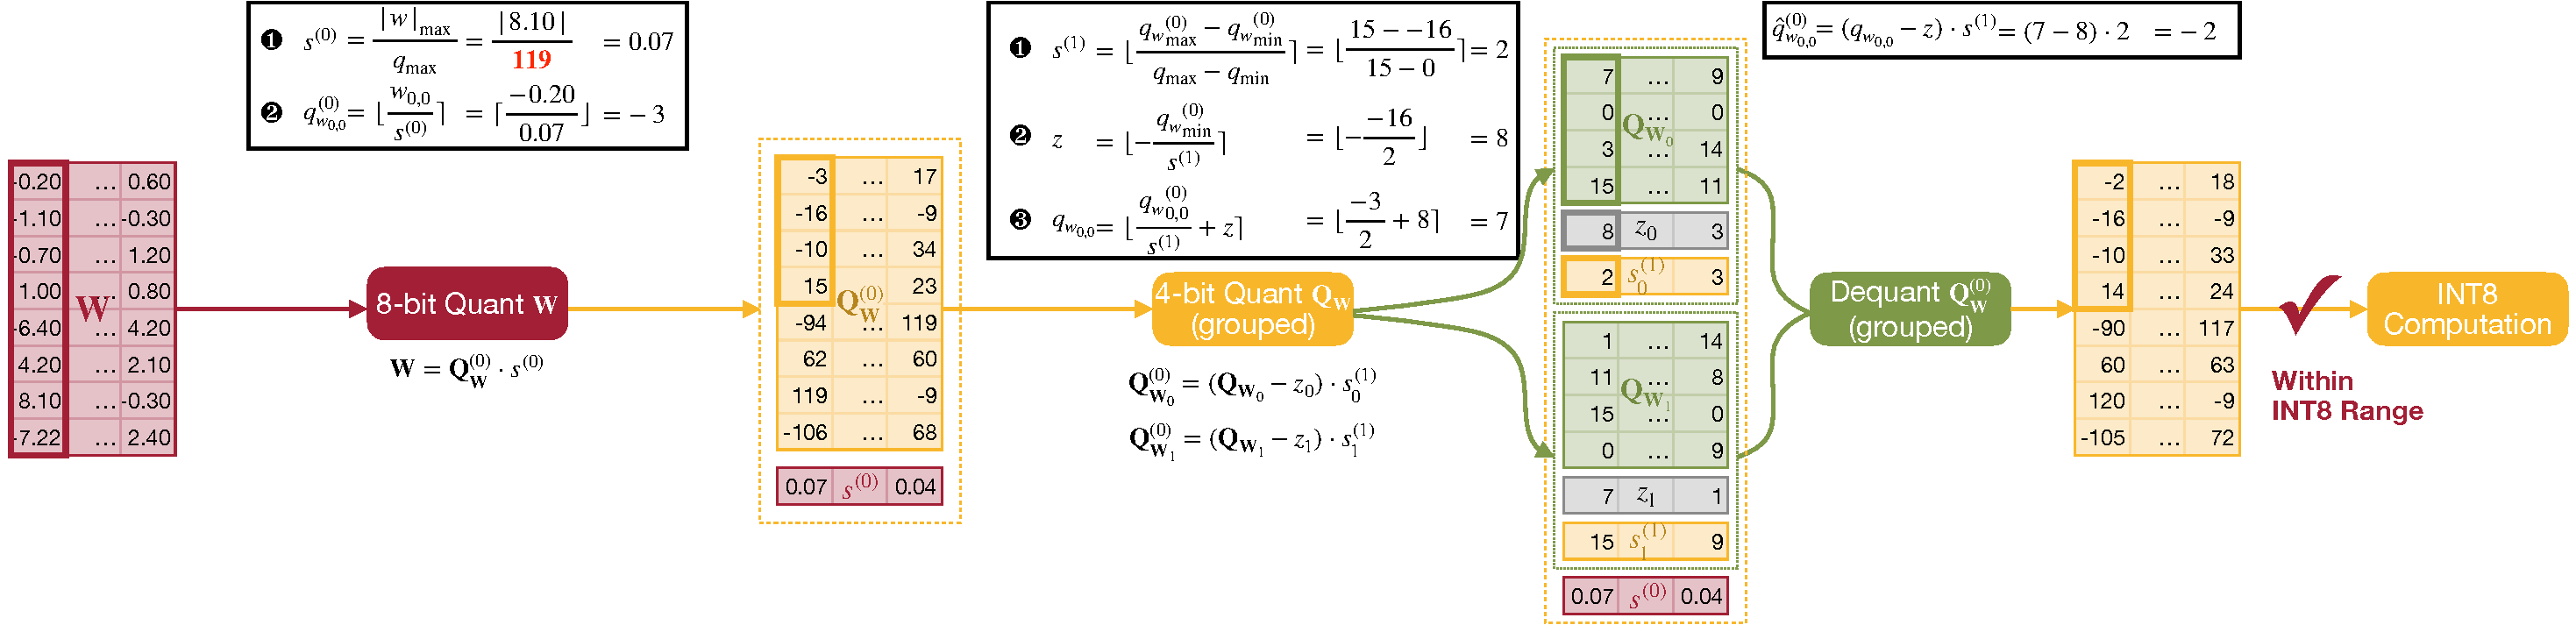
\includegraphics[width=\linewidth]{figure/4-algorithm/quant-exp-two-step.pdf}
    \vspace{-20pt}
    \caption{\textbf{Progressive Group Quantization} first employs per-channel INT8 quantization with protective range [-119, 119], followed by per-group INT4 quantization, so that the dequantized intermediate values remain within the INT8 range for computation. %
    }
    \label{fig:alg:progressive-quant}
    \vspace{-15pt}
\end{figure*}

To enhance the accuracy of low-bit quantization, \textit{group quantization} is commonly utilized~\cite{zhao2023atom,lin2023awq,gptq}. However, as outlined in Section~\ref{sect:motivation:dequantization-overhead}, the dequantization overhead in the system implementation can negate these accuracy improvements. To tackle this issue, we introduce progressive group quantization, as depicted in Figure~\ref{fig:alg:progressive-quant}.

Given the weight tensor $\mathbf{W} \in \mathbb{R}^{k \times n}$, we first apply \textit{per-channel} \textit{symmetric} \texttt{INT8} quantization:

\vspace{-10pt}
\begin{equation}
    \small \hat{\mathbf{W}} = {\mathbf{Q}_{\mathbf{W}}}^{(0)}_{\mathrm{s8}} \cdot \mathbf{s}^{(0)}_{\mathrm{fp16}},
    \label{eqn:alg:progressive_quant:int8}
\end{equation}
\vspace{-18pt}

where ${\mathbf{Q}_{\mathbf{W}}}_{\mathrm{s8}}^{(0)} \in \mathbb{N}^{n \times k}$ is the \textit{intermediate} 8-bit quantized weight tensor, and $\mathbf{s}^{(0)}_{\mathrm{fp16}} \in \mathbb{R}^{n \times 1}$ is the channel-wise quantization scales. We then further employ \textit{per-group} \textit{asymmetric} INT4 quantization on the intermediate weight tensor:

\vspace{-10pt}
\begin{equation}
 \small {{\mathbf{Q}}_{\mathbf{W}}}_\mathrm{s8}^{(0)} = \left({\mathbf{Q}_{\mathbf{W}}}_{\mathrm{u4}} - \mathbf{z}_{\mathrm{u4}} \right)\cdot \mathbf{s}^{(1)}_{\mathrm{u8}},
    \label{eqn:alg:progressive_quant:int4}
\end{equation}
\vspace{-18pt}

where ${\mathbf{Q}_{\mathbf{W}}}_{\mathrm{u4}} \in \mathbb{N}^{n \times k}$ is the unsigned 4-bit quantized weight tensor, $\mathbf{z}_{\mathrm{u4}} \in \mathbb{N}^{n \times k / g}$ is the unsigned 4-bit group-wise quantization zero points, and $\mathbf{s}^{(1)}_{\mathrm{u8}} \in \mathbb{N}^{n \times k/g}$ is the unsigned 8-bit group-wise quantization scales.

For \textbf{\texttt{W4A8}} GEMM computation, the 4-bit quantized weight tensor ${\mathbf{Q}_{\mathbf{W}}}_{\mathrm{u4}}$ will be first dequantized into intermediate 8-bit quantized weight tensor ${\mathbf{Q}_{\mathbf{W}}}_{\mathrm{s8}}^{(0)}$ following \eqn{eqn:alg:progressive_quant:int4}, and then perform \texttt{INT8} matrix multiplication as if it was \textbf{\texttt{W8A8}} per-channel quantization.

\paragraph{\textbf{Protective Quantization Range.}} Naively applying \eqn{eqn:alg:progressive_quant:int8} and~\ref{eqn:alg:progressive_quant:int4} does not guarantee that the intermediate dequantized weights perfectly lie in the 8-bit integer representation range (\ie, $[-128, 127]$). For example, after \texttt{INT8} quantization, a group of 8-bit weights lie in $[-113, 120]$. 4-bit asymmetric quantization will yield a scale factor of $\lceil (120--113)/(15-0) \rfloor =16$ and a zero point of $\lceil 0 - -113/16 \rfloor = 7$. Thus value 120 is quantized into $\lceil 120/16+7 \rfloor = 15$. It will be dequantized into $(15 - 7) * 16 = 128$ which is beyond the max 8-bit integer 127. One straightforward solution is to turn on the saturation option in the arithmetic instructions during dequantization. However, simply applying saturation will severely damage the computation throughput, reducing speed by as much as 67\%.

We reconsider the dequantization process. Take \eqn{eqn:background:quantization} into \eqn{eqn:alg:progressive_quant:int4}, we have,

\vspace{-18pt}
\begin{equation*}
    \small \hat{q}_{s8} = \lfloor \frac{{q}_{s8}}{{s}_{u8}} \rceil \cdot {{s}_{u8}} \le  {q}_{s8} + \frac{1}{2} {{s}_{u8}}
\end{equation*}
\vspace{-13pt}

Since ${s}_{u8} = \frac{{{q}_{s8}}_{\max} - {{q}_{s8}}_{\min}}{{{q}_{u4}}_{\max} - {{q}_{u4}}_{\min}} \le \frac{127-(-128)}{15-0} = 17$, we have,

\vspace{-18pt}
\begin{equation*}
    \small \hat{q}_{s8} \le 127  \rightarrow {q}_{s8} \le 127 - \frac{1}{2} {{s}_{u8}}  \rightarrow {q}_{s8} \le 119.5
\end{equation*}

\vspace{-10pt}
Therefore, we shrink the \texttt{INT8} symmetric quantization range from [-127, 127] to a \textit{protective range} [-119, 119] in order to avoid the dequantization overflow, as shown in the top of \fig{fig:alg:progressive-quant}.

\paragraph{\textbf{Compared to previous two-level quantization.}} Progressive group quantization introduces two levels of scales $\mathbf{s}^{(0)}_{\mathrm{fp16}}$ and $\mathbf{s}^{(1)}_{\mathrm{u8}}$. Prior studies such as VSQuant and DoubleQuant in QLoRA~\cite{dettmers2023qlora} also introduce two levels of scales to reduce the memory footprint of group-wise scaling factors. In contrast to our quantization flow, previous approaches directly apply group quantization with the target precision and then perform per-channel quantization on the group-wise floating-point scaling factors, as shown in the bottom of \fig{fig:alg:progressive-quant}:

\vspace{-12pt}
\begin{equation}
    \small \hat{\mathbf{W}} = {\mathbf{Q}_{\mathbf{W}}}_{\mathrm{s4}} \cdot \mathbf{s}_{\mathrm{fp16}}, \;\;\;\hat{\mathbf{s}}_{\mathrm{fp16}} = {\mathbf{s}}^{(1)}_{\mathrm{u8}} \cdot \mathbf{s}^{(0)}_{\mathrm{fp16}}
\end{equation}
\vspace{-15pt}


Therefore, using the group-wise scaling factors ${\mathbf{s}}^{(1)}_{\mathrm{u8}}$ to dequantize $\mathbf{Q}_{\mathbf{W}_{\mathrm{s4}}}$ cannot yield the 8-bit weight tensor. During the computation on GPUs, these approaches usually first dequantize the scales and, subsequently, the weights into floating-point values, which ultimately limits the peak throughput.

DGQ~\cite{zhang2023dual} also follows the quantization scheme of VSQuant and DoubleQuant, but enforces restrictions on scaling factors to make sure that all computation can be mapped onto \texttt{INT8} tensor cores. However, the DGQ serving system separates dequantization kernel with the GEMM kernel. Consequently, the end-to-end latency of \texttt{W4A8} GEMM in DGQ is even slower than the \texttt{W8A8} GEMM in cuBLAS, failing to demonstrate the memory bandwidth advantage of 4-bit weight quantization. In contrast, our \algo introduces a protective range, allowing us to fuse dequantization operations into the \texttt{W4A8} GEMM kernel with full register-level parallelism, minimizing CUDA core overhead. Thus, our \system's \texttt{W4A8} per-group GEMM achieves 1.5\x speedup over the \texttt{W8A8} cuBLAS GEMM.

\subsection{SmoothAttention}
\label{sect:alg:smooth-attention}
\begin{figure}[t]
    \centering
    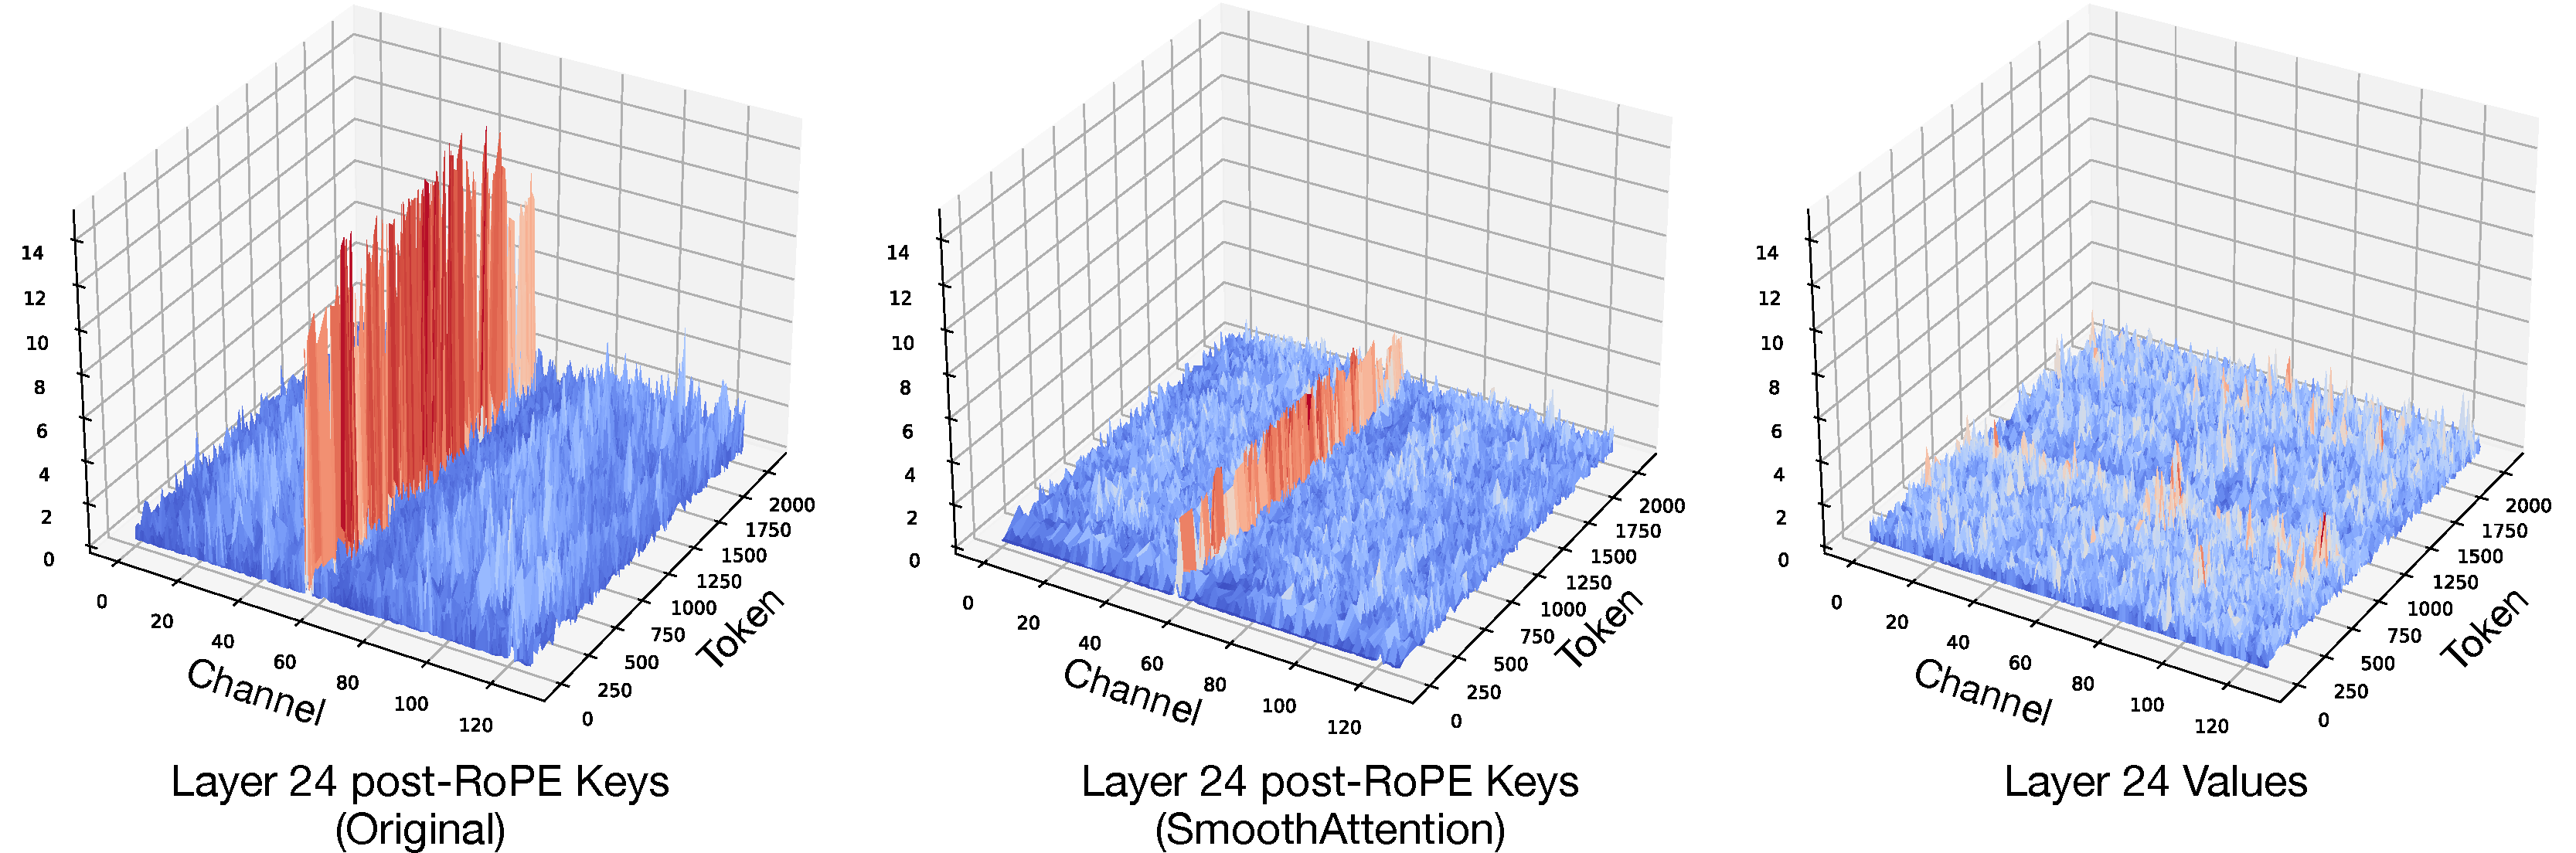
\includegraphics[width=\linewidth]{figure/4-algorithm/kvcache.pdf}
    \caption{\textbf{SmoothAttention effectively smooths the outliers in Keys. Values doesn't suffer from outliers.}}
    \label{fig:alg:smooth-attention}
    \vspace{-10pt}
\end{figure}

As illustrated in \fig{fig:evaluation:alg-ablation}, directly reducing the KV cache to 4 bits significantly degrades the LLM accuracy. We visualize the magnitude distributions of the sampled Key and Value cache activations in \fig{fig:alg:smooth-attention}. We observe that: \textbf{the Value matrices show no significant outlier pattern, whereas Key matrices tend to have fixed outlier channels in each head}. These outliers are  $\sim$10\x larger than most of activation values. Though they can be easily handled \textbf{\texttt{KV8}} quantization in prior works~\cite{xiao2023smoothquant}, it places challenging obstacle to \textbf{\texttt{KV4}} quantization due to less quantization levels.

Inspired by SmoothQuant~\cite{xiao2023smoothquant}, we propose \smoothattention to scale down the outlier channels in Key cache by a per-channel factor $\mathbf{\lambda}$:

\vspace{-10pt}
\begin{equation}
    \small \mathbf{Z} = \left(\mathbf{Q}\mathbf{\Lambda}\right)\cdot \left(\mathbf{K}\mathbf{\Lambda}^{-1}\right)^T,\;\;\;\mathbf{\Lambda}=\mathrm{diag}\left(\mathbf{\lambda}\right)
\end{equation}
\vspace{-15pt}


SmoothQuant migrates the quantization difficulty from activations to weights, and thus requires a dedicate balance between activation and weight quantization by searching the migration strength. In contrast, since we do not quantize Queries, we only need to concentrate on the Keys and simply choose the \smoothattention scale factor as,

\vspace{-10pt}
\begin{equation}
    \small \mathbf{\lambda}_{i} = \max\left(|\mathbf{K}_i|\right)^{\alpha}.
\end{equation}
\vspace{-15pt}

In practice, $\alpha=0.5$ is good enough. As shown in \fig{fig:alg:smooth-attention}, after \smoothattention, the outliers in Key cache have been greatly smoothed.

In order to eliminate the extra kernel call overhead for \smoothattention scaling, fusing the scale into preceding linear layer's weights is preferred. However, modern LLMs employ the rotary positional embedding (RoPE) to both Keys and Queries, which needs extra handling. In practice, rotary positional embedding pairs channel $i$ with channel $i+\frac{D}{2}$ within each head. Consequently, to make \smoothattention scaling commutative in terms of RoPE, we add a hard constraint that $\lambda_{i} = \lambda_{i + \frac{D}{2}}$, and accordingly,

\vspace{-15pt}
\begin{equation}
   \small \mathbf{\lambda}_{i} = \lambda_{i + \frac{D}{2}} = \max\left(\max\left(|\mathbf{K}_i|\right), \max\left(|\mathbf{K}_{i+\frac{D}{2}}|\right)\right)^{\alpha}
\end{equation}
\vspace{-15pt}

Afterwards, we can easily fuse the \smoothattention scale $\mathbf{\Lambda}$ into previous layers' weights following $\mathbf{W}_{Q} = \mathbf{\Lambda}\mathbf{W}_{Q}$ and  $\mathbf{W}_{K} = \mathbf{\Lambda}^{-1}\mathbf{W}_{K}$.


\subsection{General LLM Quantization Optimizations}
\label{sect:alg:other}
One of the key challenges of low-bit LLM quantization is the activation outliers for every linear layers. We apply different optimizations for different types of linear layers as discussed below.


\begin{figure}[t]
    \centering
    \begin{minipage}[b]{\linewidth}
    \centering
    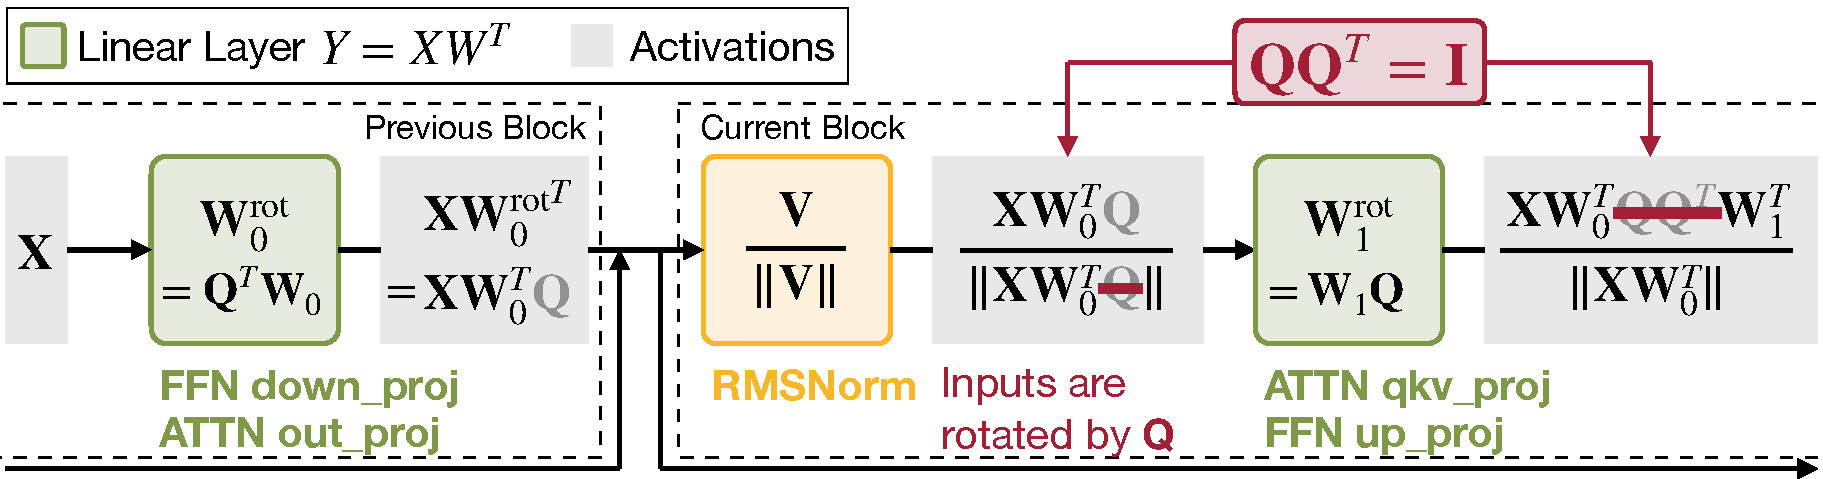
\includegraphics[width=\linewidth]{figure/4-algorithm/rotation.pdf}
    \caption{\textbf{Rotate the block input activations to suppress the outliers}: since rotation is a unitary transformation, the rotation matrix $\mathbf{Q}$ can be absorbed by the weights of the output module in the previous block.}
    \label{fig:alg:other:rotation}
    \end{minipage}
    \begin{minipage}[b]{\linewidth}
    \centering
    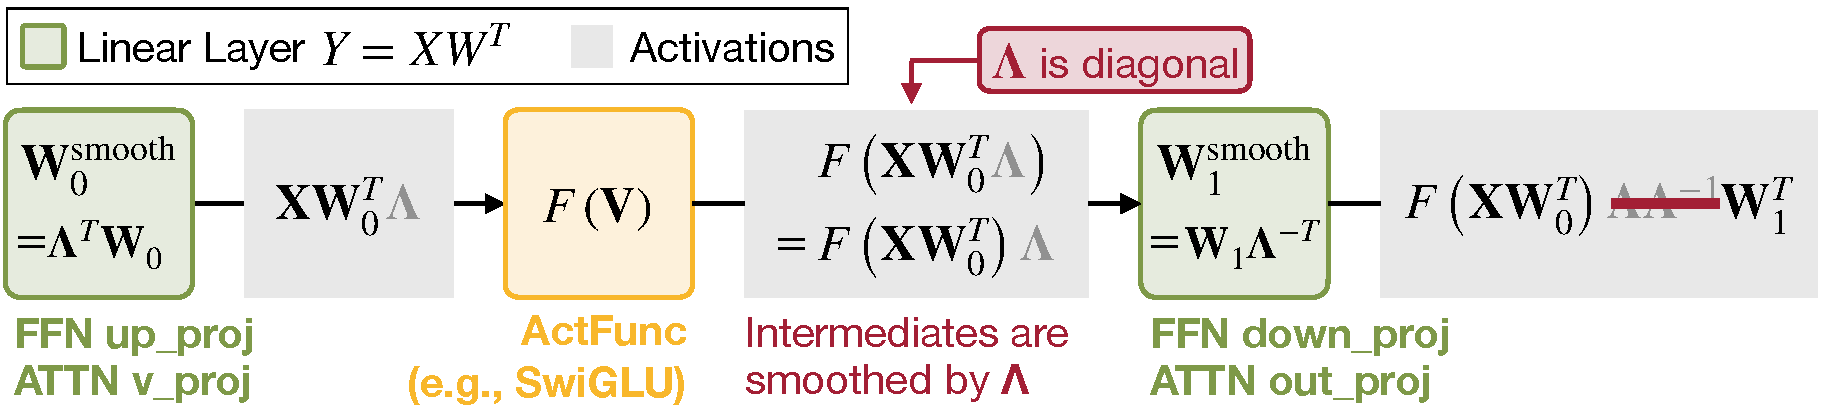
\includegraphics[width=\linewidth]{figure/4-algorithm/smooth.pdf}
    \caption{\textbf{Smooth the block intermediate activations, migrating the quantization difficulty to weights}: since smoothing is channel-independent, the smooth matrix $\mathbf{\Lambda}$ is diagonal and can be absorbed by the weights of the previous modules.}
    \label{fig:alg:other:smooth}
    \end{minipage}
\vspace{-45pt}
\end{figure}

\subsubsection{Block Input Module Rotation}
\label{sect:alg:other:rotation}
In transformer blocks, we define the components that take in the block inputs as input modules, such as the QKV Projection Layer and the FFN 1st Layer. 
As shown in \fig{fig:alg:other:rotation}, inspired by~\cite{ashkboos2024quarot,quip}, we rotate the block input activations by multiplying the rotation matrix. To keep mathematical equivalence of linear layers, we rotate the corresponding weights accordingly in the reversed direction.
After rotation, each channel's activations are linear combinations of all other channels, and thus outlier channels are effectively suppressed. Furthermore, since rotation is a unitary transformation, we can fuse the rotation matrix with the previous linear layers' weights. We simply choose the scaled Hadamard matrix as the rotation matrix.

\subsubsection{Block Output Module Smoothing}
\label{sect:alg:other:smooth}
Output modules refer to those layers that generate block outputs, such as the Output Projection Layer and FFN 2nd Layer. As shown in \fig{fig:alg:other:smooth}, inspired by~\cite{xiao2023smoothquant}, we smooth the block intermediate activations through dividing them by a per-channel smoothing factor. Original SmoothQuant does not smooth the block intermediate activations; moreover, if we directly smooth these modules with the same migration strength as input modules (\eg, \texttt{q\_proj}, \texttt{up\_proj}), the evaluated Wikitext-2 perplexity of the Llama-2-7B model will drop by as much as 0.05. In practice, we find that the migration strength $\alpha$ should be near 0. That is, the smoothing factor $\lambda$ is mostly determined by weights instead of activations, which is very different from the observations in SmoothQuant.

\subsubsection{Activation-Aware Channel Reordering}
\label{sect:alg:other:reorder}

\begin{figure}[t]
    \centering
    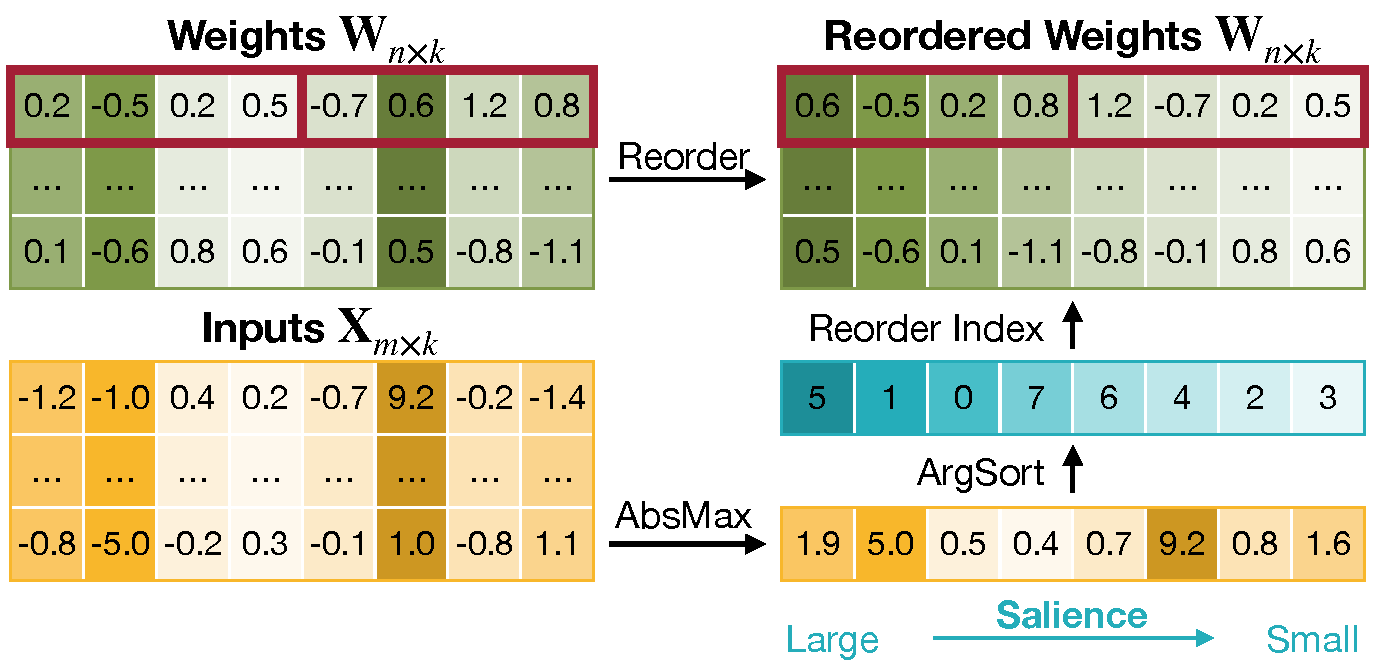
\includegraphics[width=\linewidth]{figure/4-algorithm/reorder-sequential.pdf}
    \caption{Reorder weight input channels based on their salience in group quantization. Channel salience can be determined by the magnitude of input activations.}
    \label{fig:alg:other:reorder}
\end{figure}

Both AWQ~\cite{lin2023awq} and Atom~\cite{zhao2023atom} have observed that maintaining the salient weights in FP16 can significantly improve model accuracy. These salient weights can be identified by the activation distribution. Instead of introducing mixed-precision quantization used by Atom, we propose activation-aware channel reordering as shown in \fig{fig:alg:other:reorder}. We use $\max\left(|\mathbf{X}|\right)$ to determine the channel salience, and then reorder channels so that channels with similar salience are in the same quantization group.

\subsubsection{Weight Clipping}
\label{sect:alg:other:clipping}
Weight clipping is another popular quantization optimization technique. It applies a clip ratio $\alpha$ to the dynamic range in \eqn{eqn:background:quantization} by letting $\mathbf{W}_{\max}=\alpha \max\left(\mathbf{W}\right)$ and $\mathbf{W}_{\min}=\alpha \min\left(\mathbf{W}\right)$.
Previous approaches~\cite{gptq,zhao2023atom,ashkboos2024quarot, lin2023awq} grid search the clip ratio $\alpha$ to minimize either quantization error of tensor itself (\ie, $\|\mathbf{W} - Q\left(\mathbf{W};\alpha\right)\|$) or output mean square error (\ie, $\|\mathbf{X}\mathbf{W}^T - \mathbf{X}Q\left(\mathbf{W}^T;\alpha\right)\|$. In \algo, we minimize the layer output error for all linear layers, expect for \texttt{q\_proj} and \texttt{k\_proj}, for which we optimize block output mean square error:

\vspace{-15pt}
\begin{equation}
    \small \arg\min_{\alpha} \|\mathrm{Block}\left(\mathbf{X}; \mathbf{W}\right) - \mathrm{Block}\left(\mathbf{X}; Q\left(\mathbf{W}; \alpha\right)\right)\|.
\end{equation}




